\section{Introduction}
Blabla bla.\bigskip

blabla bla.\bigskip

blabla

\section{Les triangles}

\begin{definition}[Triangle rectangle]
Un triangle rectangle est ...
\end{definition}

blabla \bigskip

blablablabla

\begin{theorem}[Pythagore]
Le carré de l'hypothénuse est égal à la somme des carrés des longueurs des 2 côtés opposés.
\end{theorem}

cf \cite{tao} pour une preuve

\subsection{sous section}

blabla
\begin{itemize}
\item une ligne
\item une autre ligne avec une formule $f(x) = ax+b$
\end{itemize}

\begin{remark}
Attention à ne rien oublier.
\end{remark}

\begin{center}
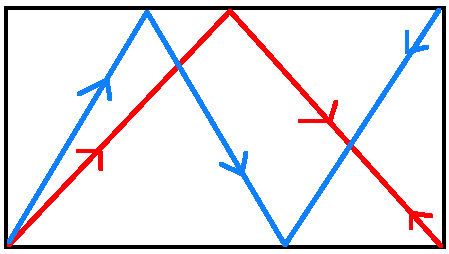
\includegraphics[width=3in,height=2.09in, clip]{images/billard.png}
\end{center}

